\section{Description des classes}
  \subsection{Ordre d'appel}
    La création d'une \bdd\ doit respecter les régles d'appel suivantes:
    \subsubsection{Création d'un objet \IGEN\ \para{Constructeur}}
      \begin{itemize}
       \item[\ding{0}] En début de programme
       \item[\ding{0}] \Cpp{\IGEN\ obj\_igen;}
       \item[\ding{0}] \Cpp{\IGEN\ obj\_igen(method, reference);}
      \end{itemize}
    \subsubsection{Paramètres \para{parametres}}
      \begin{itemize}
	\item[\ding{0}] Doit être mis avant la création des maillages
	\item[\ding{0}] \Cpp{obj\_igen.set\_method(method);}
	\item[\ding{0}] \Cpp{obj\_igen.set\_extremum(pmin,pmax,Tmin,Tmax);}
      \end{itemize}
    \subsubsection{Création des maillages \para{initm}}
      \begin{itemize}
	\item[\ding{0}] \Cpp{obj\_igen.make\_mesh(nb\_p, nb\_h, level\_max);}
      \end{itemize}
    \subsubsection{Critères de qualités \para{qualite}}
      \begin{itemize}
	\item[\ding{0}] Doit être placé avant le raffinement, 
	\item[\ding{0}] plusieurs critères de qualité peuvent être définis
	\item[\ding{0}] \Cpp{obj\_igen.set\_quality(property,type,is\_abs,limit\_qi);}
      \end{itemize}
    \subsubsection{Raffinement des maillages \para{raf}}
      \begin{itemize}
	\item[\ding{0}] Lorsque l'objet \IGEN\ est complètement paramétré
	\item[\ding{0}] \Cpp{obj\_igen.make\_global\_refine();}
	\item[\ding{0}] \Cpp{obj\_igen.make\_local\_refine();}
      \end{itemize}
    \subsubsection{Ecriture de la \bdd\ \para{ebdd}}
      \begin{itemize}
	\item[\ding{0}] Optionnel
	\item[\ding{0}] \Cpp{obj\_igen.set\_file\_med\_name(file\_med\_name);}
	\item[\ding{0}] Dernier appel 
	\item[\ding{0}] \Cpp{obj\_igen.write\_med();}
      \end{itemize}
      
    \clearpage
      
  \subsection{Classes et attributs}
    La Figure \ref{uml_att} présente la hiérarchie des classes, ainsi que le descriptif des attributs, sous la forme d'un diagramme UML:
    \begin{figure}[H]
      \center
      \includegraphics[width=1.0\textwidth]{Eos_IGen_att.eps}
      \caption{Diagramme UML des classes permettant la génération de \bdd}\label{uml_att}
    \end{figure}
    
    
